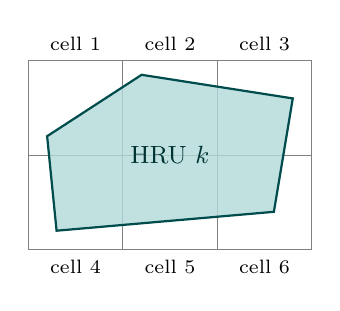
\begin{tikzpicture}[x=1.2cm,y=1.2cm]
\foreach \x in {0,1,2,3} \draw[gray] (\x,0) -- (\x,2);
\foreach \y in {0,1,2} \draw[gray] (0,\y) -- (3,\y);
\fill[teal!30,opacity=0.8] (0.3,0.2) -- (2.6,0.4) -- (2.8,1.6) -- (1.2,1.85) -- (0.2,1.2) -- cycle;
\draw[teal!60!black,thick] (0.3,0.2) -- (2.6,0.4) -- (2.8,1.6) -- (1.2,1.85) -- (0.2,1.2) -- cycle;
\node[font=\scriptsize] at (0.5,2.18) {cell 1}; \node[font=\scriptsize] at (1.5,2.18) {cell 2}; \node[font=\scriptsize] at (2.5,2.18) {cell 3};
\node[font=\scriptsize] at (0.5,-0.18) {cell 4}; \node[font=\scriptsize] at (1.5,-0.18) {cell 5}; \node[font=\scriptsize] at (2.5,-0.18) {cell 6};
\node[font=\small,teal!40!black] at (1.5,1.0) {HRU $k$};
\end{tikzpicture}
